\chapter{Artificial Neural Networks}\label{chap:ann}
This chapter will discuss the basics of artificial neural networks, which will be referenced throughout the rest of the thesis. All of the theory discussed in this chapter have been used in some way to achieve the results presented in Chapter \ref{chap:results}. This chapter will not introduce anything new to someone who is familiar with artificial neural networks.

\section{Introduction to Artificial Neural Networks}
An artificial neural network is a machine learning model inspired by biological neural networks \parencite{lippmann1987introduction}. \cite{Goodfellow-et-al-2016}, describe artificial neural networks as directed and acyclic graphs (see Figure \ref{fig:simple_ann}). They go on to say that the network is constructed of artificial neurons which are structured in layers -- these neurons are represented as nodes in a graph. Each neuron represents a function that takes some input from preceding nodes and produces an output. The input data to the network is represented by a vector $\vec{x} = [x_1, x_2, x_3, \dots, x_n]^T$ with $n$ features. The vector $\vec{x}$ could for example represent a whole sentence where $x_i$ represents a word.
\\\\
The edges in the network are connections between pairs of neurons. Each connection between two neurons have a weight. These weights will change as the network is optimised, as described in Section \ref{sec:trainingoptimisation}, and the way they change will directly impact the network's output. Updating the weights between neurons is thus a key component of how an artificial neural network works. In practice, this means that the weights should be updated so that the network gradually produces an output more similar to the desired target. 
\\\\
The input to a layer in the network is the matrix product between the output from a preceding layer and the weights between those two layers (usually with some bias term added as well). The weights are used to transform the input before it is propagated to subsequent layers. A convenient way to represent weights between two layers $j$ and $k$ is by a matrix, $W_{jk}$, where each element is the weight between a neuron in layer $k$ and a neuron in layer $j$, where $k<j$. Let $\vec{z_j}$ denote the input to layer $j$ where $W_{jk}$ are weights to layer $j$ from layer $k$ and $\vec{x_k}$ is the output from layer $k$. The vector $\vec{b}$ is a bias term that is added for more degrees of freedom. The input to layer $j$ is thus as shown in Equation \ref{eq:z}.
\begin{equation}\label{eq:z}
    \vec{z_j} = \vec{W_{jk}} \cdot \vec{x_k} + \vec{b_j}
\end{equation}
Let $\vec{y_i}$ denote the output of the layer $i$. For the first layer in the network (the input layer), $\vec{y_1}=\vec{x}$ where $\vec{x}$ is just the input data. The output, $\vec{y_i}$, of a layer $i$ is the result of applying some activation function on the input to the layer, $\vec{z_i}$, as shown in Equation \ref{eq:f_of_z}. Activation functions are described in further detail in Section \ref{activationfunction} but can in summary be seen as a way to scale the output element wise.
\begin{equation}\label{eq:f_of_z}
    \vec{y}_i = f(\vec{z}_i)
\end{equation}
During training, once the data have been propagated to the last layer, an error function will be used to measure the error of the model by comparing the final prediction with the expected output for the given input. The details about error functions can be found in Section \ref{errorfunction}. Furthermore, the results of the error functions are used when training the network, which is explained in Section \ref{sec:trainingoptimisation}. 
\\\\
Depth and width are often used to describe the shape of an artificial neural network \parencite{Goodfellow-et-al-2016}. The depth determines how many layers the network contains. The layers between input and output layer are called hidden layers. The more neurons a layer has the wider it is considered. \cite{Goodfellow-et-al-2016}, state that the reason for using multiple layers are taken from research in neuroscience. A large network (in either dimension) has more degrees of freedom which generally means that it will fit the data better, but could possibly overfit (see Section \ref{sec:overfitting}).

\begin{figure}[h]
    \centering
    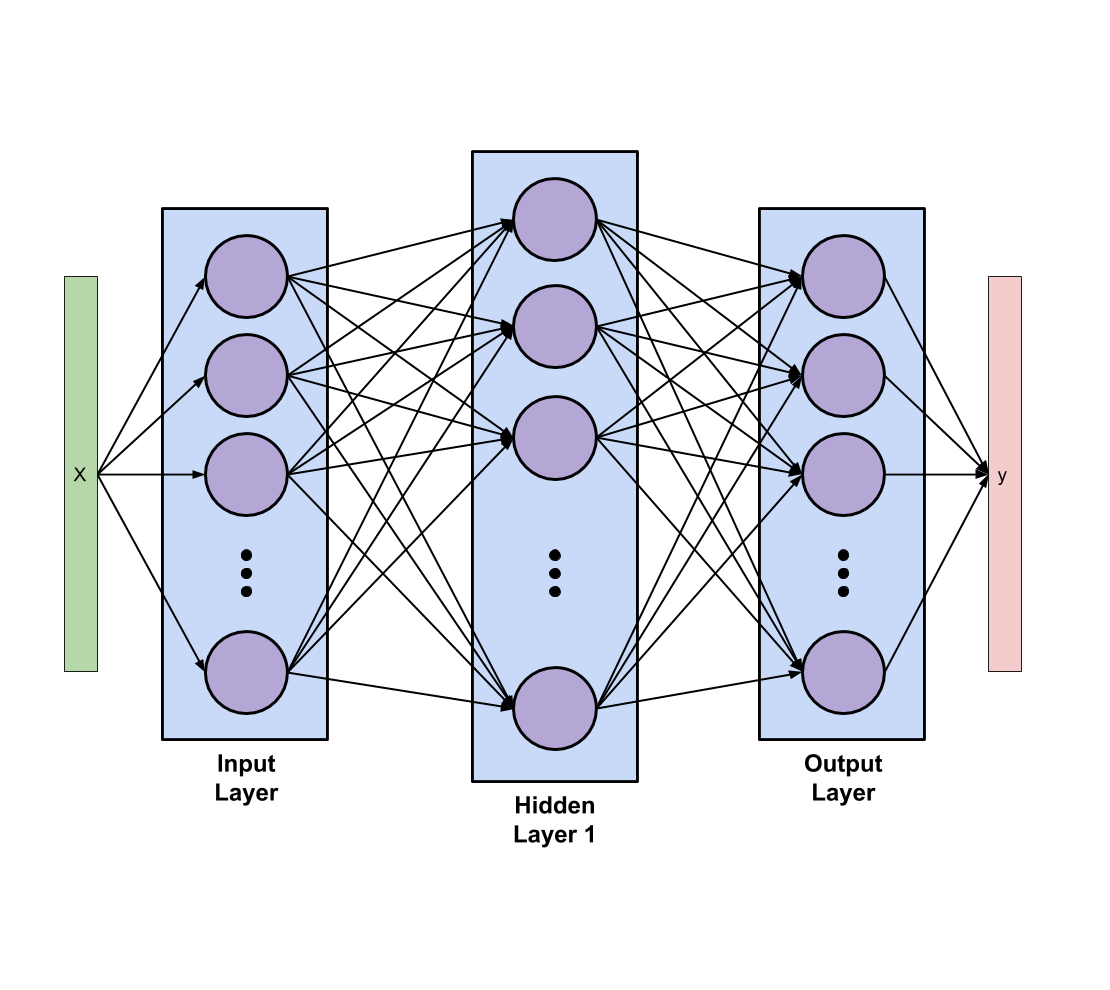
\includegraphics[width=0.75\textwidth]{figure/ann/simple_ann}
    \caption{A graph visualisation of a simple ANN. $\vec{x}$ and $\vec{y}$ are input and output vectors respectively}
    \label{fig:simple_ann}
\end{figure}

\section{Uses of Artificial Neural Networks}
A common use of machine learning is classification. It is the task of classifying a given data point as belonging to one (or more) of $k$ sets, classes, based on previously observed data \parencite{Michie94machinelearning}. Classification can be visualised as a graph of data points with curves separating $k$ groups (or \textit{classes}), these curves are also referred to as decision boundaries. For the purpose of this thesis, an artificial neural network will be used for recommending text content to users. There are however a lot of different machine learning techniques which solves the problem of automatically classifying data, e.g. Naïve Bayes Classifier \parencite{rish2001empirical}, Support Vector Machines (SVM) \parencite{boser1992training, cortes1995support}, or Decision Tree Classifier \parencite{safavian1991survey}.
\\\\
Classification of data typically requires extraction of features that can be compared. Feature engineering, as this is called, is a process that usually requires extensive domain knowledge. When using artificial neural networks, the process of feature engineering can be omitted, thus making it easier to model more complex problems \parencite{nlp2011ronan, lecun2015deep}. This property of artificial neural networks makes them suitable for many tasks. One example is to model sequences of text as it is not necessary to manually find features in the text that could be used for classification, which motivates their usage in this project.

\section{Activation Functions}\label{activationfunction}
The activation function scales the output from a node to create a new signal that is sent to the next layer \parencite{basheer2000artificial}. By using non-linear functions it is possible to scale the output, and find non-linear decision boundaries which allow better fitting to the data \parencite{lippmann1987introduction, basheer2000artificial}. Different activation functions can be used for different purposes in the same artificial neural network, it is not necessary to choose only one. In this project a few different activation functions have been used, and are described below.

\subsection{Logistic Function}\label{sec:sigmoid_function}
The logistic function is a non-linear function with an \textit{S} shaped curve, as defined by Equation \ref{eq:sigmoid}, that squashes the input, $z_j$ from Equation \ref{eq:z}, between $[0, 1]$.
\begin{equation}\label{eq:sigmoid}
    f(\vec{x})=\frac{1}{1+exp(\vec{-x})}
\end{equation}
In this project, the logistic function has been used in the final layer of the model as the output function as it is possible to interpret its output as probabilities. This particular function is especially useful for multi-label classifications (where some input can be classified as belonging to more than one class, e.g. being interesting to more than one users). When using the logistic function like this it is common to use the negative log-likelihood error function since this is particularly useful for multi-label classifications \parencite{bishop1995neural}.

\subsection{Rectified Linear Unit Function}\label{sec:relu}
The Rectified Linear Unit (ReLU) function is a non-linear function defined in Equation \ref{eq:ReLU}. This function has the benefit of being unbounded as opposed to the logistic function, which ranges in the interval $[0, 1]$. The ReLU function has become popular in the past few years due to it being less susceptible to vanishing gradient compared to other activation functions \parencite{glorot2011deep, lecun2015deep}.
\begin{equation}\label{eq:ReLU}
    f(x) = max(0,x)
\end{equation}
The ReLU function was used as the activation function in the hidden layers of the model.

\subsection{Softmax Function}\label{sec:softmax_function}
The softmax function is defined in Equation \ref{eq:softmax} where $\vec{x}$ is a vector of $n$ elements. Softmax scales the vector entries to be between $[0,1]$, while normalising them all to sum to 1.
\begin{equation} \label{eq:softmax}
    f(\vec{x}_j) = \frac{e^{\vec{x}_j}}{\sum_{i=1}^{n} e^{\vec{x}_i}}
\end{equation}
When using the softmax function in the final layer of the network to create an output it has been shown that using the cross entropy error function together with softmax gives a better accuracy compared to other error functions \parencite{dunne1997pairing,golik2013cross}. By using the softmax activation function, the output can be interpreted as normalised probabilities between the $n$ output classes. Because of the normalisation this becomes useful for classification where there is only one correct class. Softmax is used during pre-training of the network and tested as an output function for the whole model (see Section \ref{sect:enhacing_the_model}).

\section{Error Functions} \label{errorfunction}
The error function in artificial neural networks are used to compare the network's predicted output with the correct output, for a given input. When training the network, the difference between the predicted and correct output is used to minimise the error (more details in Section \ref{sec:trainingoptimisation}). There are primarily two different error functions that are used and evaluated in this thesis. For the error functions described below, $y_k$ indicates the $k^{th}$ prediction of the network, $t_k$ indicates the correct value of the $k^{th}$ prediction, and $K$ is the number of classes.
\\\\
One of the error functions examined is the cross entropy error function. It is commonly used when working with artificial neural networks because of its overall performance, compared to alternatives, when performing backpropagation (see Section \ref{sec:backpropagation} for details on backpropagation). The cross entropy function is defined in Equation \ref{eq:cross_entropy} \parencite{bishop2006crossEn}.
\begin{equation} \label{eq:cross_entropy}
    E_K = -\sum_{k=1}^{K} [t_k \cdot ln(y_k) +(1-t_k)ln(1-y_k) ]
\end{equation}
The reason behind the cross entropy function's popularity is that the derivative with respect to the weights is proportional to the difference between the predicted value and actual value, leading to better performance of the network \parencite{nasr2002cross}.
\\\\
The other error function that is evaluated is the Negative Log-Likelihood (sometimes called multi-class cross entropy) function \parencite{bishop2006pattern}. This error function, defined in Equation \ref{eq:neg_log_likelihood} \parencite{tensorflow2016cross}, could be interpreted as a more general version of the cross cntropy function. It is more suitable for multi-label classification problems compared to the Cross Entropy function which is more suitable for single-label classifications.
\begin{equation} \label{eq:neg_log_likelihood}
    E_K = \vec{t} -log(\vec{y}) + (1-\vec{t}) -log(1-\vec{y})
\end{equation}
In this project the Negative Log-Likelihood function is used as the error function when using the logistic function (see equation \ref{eq:sigmoid}) as output function for the network.

\section{Training and Optimisation} \label{sec:trainingoptimisation}
Training and optimisation in machine learning is the process of learning from data. The way a certain machine learning model learns from data usually differs but the training of an artificial neural network can be seen as a problem of optimising the network's weights. For this to work, an error function is needed that determines how much a certain prediction for a data point is wrong compared to the true classification of that data point. The optimisation objective is to find the weights and biases in the artificial neural network that minimises the error for the training data. This can be achieved by applying backpropagation and some optimisation method, e.g. Gradient descent (see Section \ref{sec:gradient_descent}). The process of learning from some previously classified data is called supervised learning \parencite{lecun2015deep}. This training process is required to improve the performance of  the artificial neural network. \parencite{Goodfellow-et-al-2016}.

\subsection{Gradient Descent Optimisation}\label{sec:gradient_descent}
Gradient descent is an iterative algorithm where the gradient of a function is calculated in steps. The computed gradient is used to move towards the minimum of the function. This is repeated until a local or global minimum of the function is found. Computing the gradient for the whole dataset is computationally heavy. This leads to that the datasets used for training are divided into small batches, minibatches. When using minibatches, the gradients of the error function for each data point in the minibatch is computed and then averaged to approximate the full gradient. When applying gradient descent to this approximation it is known as stochastic gradient descent. It has been shown that stochastic gradient descent is fast for convex functions \parencite{convexSGD}. There are no guarantees that an artificial neural network will be convex, but there is a specialised and efficient implementation of stochastic gradient descent called \textit{Adam} \parencite{adamoptimizer} that is commonly used for artificial neural networks. The Adam optimiser is used in this project to optimise the weights and biases of the artificial neural network model to give a minimal error. By minimising the error the predictions of the network should improve, if the model is working.

\subsection{Using Backpropagation}\label{sec:backpropagation}
Backpropagation is a method used for training artificial neural networks. When you feed an input vector (e.g. a sentence) to the network, the network will propagate the vector forward until it reaches the last layer and presents a prediction. The prediction is then compared to the desired result for the given input via an error function to determine how well the network performed. The error is propagated backwards through the network to determine how much every individual weight and bias impacted it. The weights and biases for each neuron is then updated accordingly. How the weights and biases are updated depends on which optimisation method is used. This training is performed on all of the data points in a training data. Each training iteration over the complete set of data is called an epoch.

\subsection{Overfitting}\label{sec:overfitting}
Overfitting can be described by a state of the model where the network does not generalise well, meaning that the network is too specialised on the training data. This phenomenon results in bad accuracy of the network when it is faced with previously unseen data. This is a common problem if the network has too many parameters that can describe the training data instead of capturing the general idea of the data.
\begin{figure}[h]
    \centering
    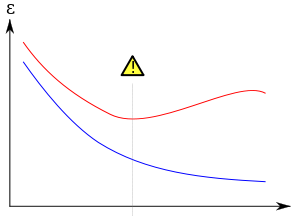
\includegraphics[width=0.5\textwidth]{figure/ann/overfitting}
    \caption{An example of overfitting. The red line shows the error on the validation data and the blue line shows the error on the training data. It is desired that the error is as low as possible. 
    "\href{https://en.wikipedia.org/wiki/Overfitting\#/media/File:Overfitting_svg.svg}{Overfitting}" by
    \href{https://commons.wikimedia.org/wiki/User:Gringer}{Gringer}, edited by
    \href{https://commons.wikimedia.org/wiki/User\:Dake}{Dake}, is licensed under CC-BY 3.0.}
    \label{fig:overfitting}
\end{figure}
\\
As seen in Figure \ref{fig:overfitting} the network is performing better and better for both training and validation sets. However, it reaches a point where the validation error starts going up. That point is where the overfitting has occurred. The training error is still decreasing meaning that the network keeps learning on the training data instead of generalising from it. 

\subsection{Regularisation}\label{sec:regularisation}
Regularisation is a set of techniques used in order to prevent the overfitting problem described in Section \ref{sec:overfitting}. These techniques increase the performance of the network as they allow the network to continue generalising without overfitting, at the cost of sometimes limiting the networks. In this thesis two different regularisation techniques have been used:
\begin{itemize}
    \item Dropout
    \item $l^2$-loss regularisation
\end{itemize}
\\\\
Dropout is a rather newly discovered regularisation technique that prevents overfitting by randomly disabling neurons in the artificial neural network \parencite{srivastava2014dropout}. During the training of the network, neurons are randomly disabled with a probability $p$. This means that the network has to teach other neurons to do the generalisation that the disabled neuron previously did. It is important to note that this is only used during the training of the network. When validating the performance of the network or actually using the network all neurons are used.
\\\\
The purpose of $l^2$-loss regularisation is to prevent weights from becoming extremely large by penalising them based on their size. The $l^2$ regularisation is used by adding the $l^2$-norm of every weight in the artificial neural network to the error function. The penalisation leads to a limitation in the network's capacity, or \textit{statistical complexity}, in terms of the $l^2$-norm \parencite{neyshabur2015norm}. 
\\\\
A powerful aspect of these two regularisation techniques is that they work alongside each other. This is because they are implemented in different parts of the artificial neural network model.

\section{Recurrent Neural Networks }\label{sec:rnn}
A recurrent neural network (RNN) is an artificial neural network that takes context into account. It accounts for context in the sense that the current output is dependent on the previous. This context dependency is often depicted as an artificial neural network that has its own output as input, in practice however, recurrent neural networks are instead modelled as chained (or \textit{unfolded}) \textit{units} as shown in Figure \ref{fig:chained_units}. A unit takes two inputs; the output from the previous unit and input data. The output produced is passed along to the next unit but could also be retrieved and used. An arbitrary number of units can be chained in this way but in this project the number of units will be related to the length of the input text. 
\begin{figure}[h!]
    \centering
    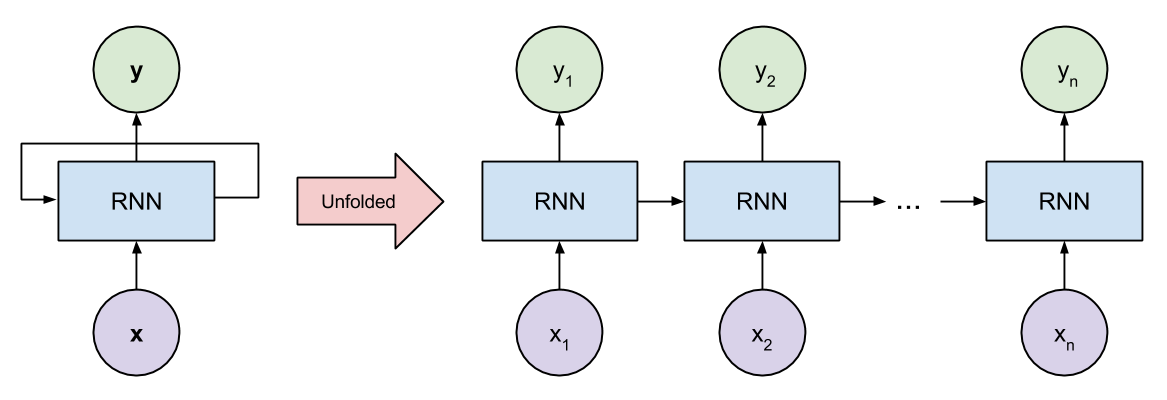
\includegraphics[width=0.95\textwidth]{figure/ann/rnn_unfold}
    \caption{A visualisation of a recurrent neural network layer and how it is unfolded. $\vec{x}$ and $\vec{y}$ are the input and output vector respectively}
    \label{fig:chained_units}
\end{figure}
\\\\
Recurrent neural networks are particularly useful when modelling with natural language as input since words in a sentence often are dependent on what comes before them. When using sentences as input, it is common to have one word as input per unit in the recurrent neural network \parencite{palangi2016deep}. This is how recurrent neural networks were used in this project to model social platform content.
\\\\
The units in a recurrent neural network can be implemented in different ways. Popular unit implementations are Long Short Term Memory (LSTM) and Gated Recurrent Unit (GRU). The LSTM unit was introduced to solve the problems of inefficiency in the backpropagation for recurrent neural networks \parencite{LSTMdefined}. The inefficiencies occurred because the error gradient would decay and approach zero, making training very slow, and this is what the LSTM solves \parencite{hochreiter1998vanishing}. The GRU unit is a fairly recent addition to the field and it is comparable to the LSTM in accuracy, but the dataset used can have a big impact on which one performs better \parencite{GRUchung2014empirical}. The fact that either of the unit implementations might perform better based on the dataset used motivates testing them both in this thesis.

\subsection{Using Recurrent Neural Networks for Natural Language Processing}\label{sec:rnn_nlp}
As previously mentioned, when working with natural language it is common to let every unit in a recurrent neural network layer take one word as input. This is illustrated in Figure \ref{fig:sentence_to_rnn} below.
\begin{figure}[h]
    \centering
    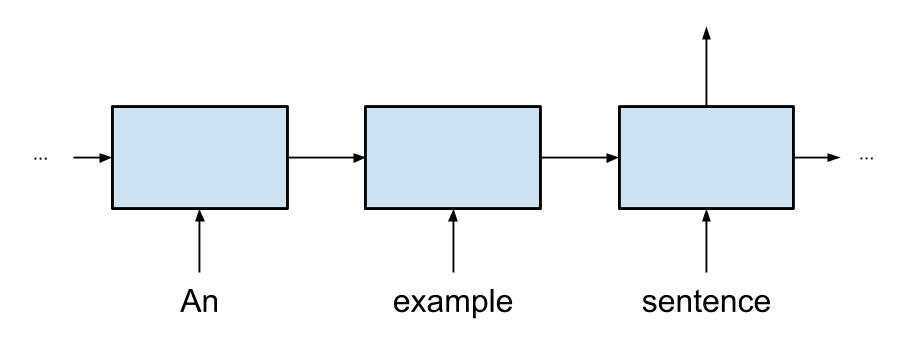
\includegraphics[width=0.75\textwidth]{figure/ann/sentence_to_rnn}
    \caption{A simplification of how a recurrent neural network layers process natural language as input}
    \label{fig:sentence_to_rnn}
\end{figure}
\\
The units however, just as an artificial neural network, expect some vector as input. This means that the input sentences have to be transformed into vectors. A common way to achieve this is to use indices instead of strings of words. With this approach each unique word is given a unique number, and an input sentence of words then become a vector of word indices. It is also common to take the transformation one step further and turn each word index into a so called one-hot vector \parencite{turian2010word}. Using one-hot vectors, each word is represented as a vector $\vec{w}$ of length $C$, where $C$ represents the total number of words, having a $1$ at the position of the given word's index and zeros everywhere else (this is illustrated by Table \ref{tab:onehot}). Since the length of the vector is fixed, it means that new words that are not in the known set of words, the vocabulary, can not be represented as a one-hot vector -- to solve this, new words are represented together as \textit{unknown} (usually with an index of $0$). 
\begin{table}[h!]
    \centering
    \begin{tabular}{c|c}
    \textbf{Word} & \textbf{Vector representation} \\
    \hline \hline
    This & $[0, 0, 0, 0, 1]^T$ \\ \hline
    is & $[0, 0, 1, 0, 0]^T$ \\ \hline
    a & $[0, 1, 0, 0, 0]^T$ \\ \hline
    normal & $[0, 0, 0, 1, 1]^T$ \\ \hline
    sentence & $[1, 0, 0, 0, 0]^T$ \\ \hline
    \end{tabular}
    \caption{An illustration of the sentence "This is a normal sentence" using one-hot vectors, given that the vocabulary is \{\textit{unknown}, a, is, normal, this\}.}
    \label{tab:onehot}
\end{table} 
\\\\
Another problem with one-hot vectors is that they do not hold any information about relationships between words. This motivates using another representation for words in order to capture the connection. This can be done with algorithms such as word2vec \parencite{mikolov2013linguistic} or GloVe \parencite{pennington2014glove}, which produce so called \textit{embedding matrices}.